\begin{tiny}Cfu05\end{tiny} \label{ineqtrig1} Utilisons la méthode du cours pour transformer une combinaison linéaire trigonométrique
\begin{multline*}
  a \cos \theta + b \sin \theta \\
  = \sqrt{a^2 + b^2}\left( \frac{a}{\sqrt{a^2 + b^2}}\cos \theta + \frac{b}{\sqrt{a^2 + b^2}}\sin \theta\right).
\end{multline*}
Ici
\begin{multline*}
  \sqrt{3}\cos \theta - \sin \theta = 2 \left( \frac{\sqrt{3}}{2} \cos \theta - \frac{1}{2}\sin \theta\right)\\
  = 2 \left( \cos \frac{\pi}{6} \cos \theta -\sin \frac{\pi}{6} \sin \theta\right)
  = 2 \cos(\theta + \frac{\pi}{6}).
\end{multline*}
L'inéquation est donc équivalente à 
\[
  \cos(\theta + \frac{\pi}{6}) \leq \frac{1}{2}.
\]
\begin{figure}[h!]
  \centering
  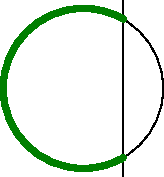
\includegraphics{Cfu05_1.pdf}
  % Cfu05_1.pdf: 113x113 px, 72dpi, 3.99x3.99 cm, bb=0 0 113 113
  \label{fig:Cfu05_1}
  \caption{Exercice \ref{ineqtrig1} fu05}
\end{figure}
Pour $\theta + \frac{\pi}{6}$ entre $0$ et $2\pi$, l'inéquation est vérifiée si (\ref{fig:Cfu05_1})
\[
  \frac{\pi}{3} \leq \theta + \frac{\pi}{6} \leq 2\pi - \frac{\pi}{3}
  \Leftrightarrow
 \theta \in \left[\frac{\pi}{6} , \frac{3\pi}{2} \right].
\]
Par périodicité, pour tout $k\in \Z$, on peut ajouter $2k\pi$ à cet intervalle. 
